% ******************************************************
% A Classic Thesis Style
% An Homage to The Elements of Typographic Style
%
% Copyright (C) 2018 André Miede and Ivo Pletikosić
% ******************************************************
\RequirePackage{silence}
    \WarningFilter{scrreprt}{Usage of this version of package `titlesec'}
    \WarningFilter{scrreprt}{Usage of package `tocloft' together}
    \WarningFilter{titlesec}{Non standard sectioning command}
\documentclass[% TODO: go through these
    twoside,
    openright,
    titlepage,
    numbers=noenddot,
    %1headlines,
    headinclude,
    footinclude,
    cleardoublepage=empty,
    abstract=on,
    BCOR=5mm,
    paper=a4,
    fontsize=11pt
]{scrreprt}

% ******************************************************
% Note: Make all your adjustments in here
% ******************************************************
\PassOptionsToPackage{utf8}{inputenc}
\usepackage{inputenc}

\PassOptionsToPackage{T1}{fontenc}
\usepackage{fontenc}


% ********************************************************************
% 1. Configure classicthesis for your needs here, e.g., remove "drafting" below
% in order to deactivate the time-stamp on the pages
% (see ClassicThesis.pdf for more information):
% ********************************************************************
\PassOptionsToPackage{
    drafting=true,    % print version information on the bottom of the pages
    tocaligned=false, % the left column of the toc will be aligned (no indentation)
    dottedtoc=false,  % page numbers in ToC flushed right
    eulerchapternumbers=true, % use AMS Euler for chapter font (otherwise Palatino)
    linedheaders=false,       % chaper headers will have line above and beneath
    floatperchapter=true,     % numbering per chapter for all floats (i.e., Figure 1.1)
    eulermath=false,  % use awesome Euler fonts for mathematical formulae (only with pdfLaTeX)
    beramono=true,    % toggle a nice monospaced font (w/ bold)
    palatino=true,    % deactivate standard font for loading another one, see the last section at the end of this file for suggestions
    style=classicthesis % classicthesis, arsclassica
}{classicthesis}


% ********************************************************************
% 2. Personal data and user ad-hoc commands (insert your own data here)
% ********************************************************************
\newcommand{\myTitle}{Quantum Circuit Compilation From The Ground Up\xspace}
\newcommand{\mySubtitle}{\xspace}
\newcommand{\myDegree}{Master of Mathematics (MMath)\xspace}
\newcommand{\myName}{Nathaniel Stemen\xspace}
% \newcommand{\myProf}{Someone else TODO\xspace}
\newcommand{\mySupervisor}{Joel Wallman\xspace}
\newcommand{\myFaculty}{Faculty of Mathematics\xspace}
\newcommand{\myDepartment}{Department of Applied Mathematics\xspace}
\newcommand{\myUni}{University of Waterloo\xspace}
\newcommand{\myInst}{Institute for Quantum Computing\xspace}
\newcommand{\myLocation}{Seattle, WA\xspace}
\newcommand{\myTime}{April 2022\xspace}
\newcommand{\myTimeFrame}{September 2020---April 2022}
\newcommand{\myVersion}{\classicthesis}

% ********************************************************************
% 3. Loading some handy packages
% ********************************************************************

% ********************************************************************
% Packages with options that might require adjustments
% ********************************************************************
\PassOptionsToPackage{american}{babel}
\usepackage{babel}

\usepackage{csquotes}

\PassOptionsToPackage{
    style=alphabetic,
    maxnames=5,
    backref=true
}{biblatex}
\usepackage{biblatex}

\PassOptionsToPackage{fleqn}{amsmath} % float equations towards left side
\usepackage{amsmath}
\usepackage{amssymb}
\newtheorem{theorem}{Theorem}[section]
\newtheorem{definition}[theorem]{Definition}
\newtheorem{example}[theorem]{Example}
\newtheorem{question}[theorem]{Question}

% ********************************************************************
% General useful packages
% ********************************************************************
\usepackage{graphicx}
\usepackage{scrhack} % fix warnings when using KOMA with listings package
\usepackage{xspace} % to get the spacing after macros right
\PassOptionsToPackage{printonlyused,smaller}{acronym}
\usepackage{acronym} % TODO change to acro package
\usepackage{physics}
\usepackage{mathtools}
\usepackage{stmaryrd}
\DeclarePairedDelimiter\implement{\llbracket}{\rrbracket}
\usepackage{xfrac}


% ********************************************************************
% 4. Setup floats: tables, (sub)figures, and captions
% ********************************************************************
\usepackage{tabularx} % better tables: TODO change to booktabs
\setlength{\extrarowheight}{3pt} % increase table row height
\newcommand{\tableheadline}[1]{\multicolumn{1}{l}{\spacedlowsmallcaps{#1}}}
\newcommand{\myfloatalign}{\centering} % to be used with each float for alignment
\usepackage{subfig}


% ********************************************************************
% 5. Setup code listings
% ********************************************************************
\usepackage{listings}
%\lstset{emph={trueIndex,root},emphstyle=\color{BlueViolet}}%\underbar} % for special keywords
\lstset{language=[LaTeX]Tex,%C++,
    morekeywords={PassOptionsToPackage,selectlanguage},
    keywordstyle=\color{RoyalBlue},%\bfseries,
    basicstyle=\small\ttfamily,
    %identifierstyle=\color{NavyBlue},
    commentstyle=\color{Green}\ttfamily,
    stringstyle=\rmfamily,
    numbers=none,%left,%
    numberstyle=\scriptsize,%\tiny
    stepnumber=5,
    numbersep=8pt,
    showstringspaces=false,
    breaklines=true,
    %frameround=ftff,
    %frame=single,
    belowcaptionskip=.75\baselineskip
    %frame=L
}


% ********************************************************************
% 6. Last calls before the bar closes
% ********************************************************************
\usepackage{classicthesis}


% ********************************************************************
% Fine-tune hyperreferences (hyperref should be called last)
% ********************************************************************
\hypersetup{%
    % COLOR ***********
    colorlinks=true,
    linktocpage=true,
    urlcolor=CTurl, linkcolor=CTlink, citecolor=CTcitation,
    % urlcolor=Black, linkcolor=Black, citecolor=Black, % for printing
    % IDK TBH *********
    breaklinks=true,
    pageanchor=true,
    bookmarksnumbered=true, bookmarksopen=true, bookmarksopenlevel=1,
    % PDF META ********
    pdftitle={\myTitle},
    pdfauthor={\textcopyright\ \myName, \myUni},
    pdfsubject={Quantum Circuit Compilation},
    pdfkeywords={quantum information, quantum computation, quantum circuits, compilers},
    pdfcreator={pdfLaTeX},
    pdfproducer={LaTeX with hyperref and classicthesis},
}


% ********************************************************************
% Setup autoreferences (hyperref and babel)
% ********************************************************************
% There are some issues regarding autorefnames
% http://www.tex.ac.uk/cgi-bin/texfaq2html?label=latexwords
% you have to redefine the macros for the
% language you use, e.g., american, ngerman
% (as chosen when loading babel/AtBeginDocument)
% ********************************************************************
\makeatletter
\@ifpackageloaded{babel}%
{%
    \addto\extrasamerican{%
        \renewcommand*{\figureautorefname}{Figure}%
        \renewcommand*{\tableautorefname}{Table}%
        \renewcommand*{\partautorefname}{Part}%
        \renewcommand*{\chapterautorefname}{Chapter}%
        \renewcommand*{\sectionautorefname}{Section}%
        \renewcommand*{\subsectionautorefname}{Section}%
        \renewcommand*{\subsubsectionautorefname}{Section}%
    }%
    % Fix to getting autorefs for subfigures right (thanks to Belinda Vogt for changing the definition)
    \providecommand{\subfigureautorefname}{\figureautorefname}%
}{\relax}
\makeatother


\newcommand{\R}{\mathbb{R}}
\newcommand{\C}{\mathbb{C}}
\newcommand{\F}{\mathbb{F}}
\newcommand{\1}{\mathbb{1}}
\newcommand{\iu}{\mkern1mu\mathrm{i}\mkern1mu}
\newcommand{\e}{\mathrm{e}}
\newcommand{\mats}[2]{\mathcal{M}_{#1}(#2)}
\newcommand{\U}[1]{\mathsf{U} (#1)}
\newcommand{\PU}[1]{\mathsf{PU} (#1)}

\newcommand{\CNOT}{\ensuremath{\mathsf{CNOT}}}
\newcommand{\CCNOT}{\ensuremath{\mathsf{CCNOT}}}
\newcommand{\SWAP}{\ensuremath{\mathsf{SWAP}}}
\newcommand{\controlled}[1]{\ensuremath{\mathsf{Controlled}\text{-}#1}}

\newcommand{\free}[1]{\expval{#1}}

\newcommand{\defeq}{\coloneqq}%\stackrel{\text{\tiny def}}{=}}
\newcommand{\eqdef}{\eqqcolon}%\stackrel{\text{\tiny def}}{=}}
\DeclareMathOperator{\vectorize}{vec}
\DeclareMathOperator{\qubits}{qubits}
\DeclareMathOperator{\End}{End}
\DeclareMathOperator*{\argmin}{arg\,min}
\DeclareMathOperator{\Fid}{F}


% Non math
\newcommand{\ie}{i.\,e.}
\newcommand{\Ie}{I.\,e.}
\newcommand{\eg}{e.\,g.}
\newcommand{\Eg}{E.\,g.}

\def\CPP{{C\nolinebreak[4]\raisebox{.15ex}{++}}}

\usepackage{tikz}
\usetikzlibrary{arrows,shadows,positioning,fit}
\usetikzlibrary{quantikz}

\usepackage[style=super]{glossaries}
\newglossary*{symbols}{List of Symbols}
\makeglossaries

\usepackage{attrib}
\usepackage{cleveref}
\usepackage{enumitem}
\usepackage{qtree}

\usepackage{todonotes}

\newlist{requirements}{enumerate}{10}
\setlist[requirements]{label*=\arabic*}
\crefname{requirementsi}{requirements}{requirements}
\Crefname{requirementsi}{Requirements}{Requirements}

% ******************************************************
% Bibliographies
% ******************************************************
\addbibresource{bib.bib}

% ******************************************************
% Hyphenation
% ******************************************************
%\hyphenation{put special hyphenation here}

% ******************************************************
% GO!GO!GO! MOVE IT!
% ******************************************************
\begin{document}
\frenchspacing
\raggedbottom
\selectlanguage{american}
\pagenumbering{roman}
\pagestyle{plain}
% ******************************************************
% Frontmatter
% ******************************************************
\begin{titlepage}
    \begin{addmargin}[-1cm]{-3cm}
        \begin{center}
            \large

            \hfill

            \vfill

            {
                \color{CTtitle}\spacedallcaps{\myTitle} \\ \bigskip
            }

            \spacedlowsmallcaps{\myName}

            \vfill

            \includegraphics[width=6cm]{img/uwlogo} \\ \medskip

            \myDegree \\
            \myDepartment \\
            \myFaculty \\
            \myInst \\
            \myUni \\ \bigskip

            \myTime

            \vfill

        \end{center}
    \end{addmargin}
\end{titlepage}

\thispagestyle{empty}

\hfill

\vfill

\noindent\myName: \textit{\myTitle,} \myDegree,
\textcopyright\ \myTime

\bigskip

\noindent\spacedlowsmallcaps{Supervisors}: \\
\mySupervisor

\medskip

\noindent\spacedlowsmallcaps{Location}: \\
\myLocation (completed remotely during COVID-19)

\medskip

\noindent\spacedlowsmallcaps{Time Frame}: \\
\myTimeFrame

\cleardoublepage\include{aux/dedication}
% \cleardoublepage\include{aux/foreword}
\cleardoublepage% ******************************************************
% Abstract
% ******************************************************
%\renewcommand{\abstractname}{Abstract}
\pdfbookmark[1]{Abstract}{Abstract}

\begingroup
\let\clearpage\relax
\let\cleardoublepage\relax
\let\cleardoublepage\relax

\chapter*{Abstract}

This thesis details the problem of quantum circuit compilation.
Starting from the very definition of compile, we introduce many of the ideas needed to understand the main problem of circuit compilation from the very basics.
We cover classical compilers and show how the effort to build effective circuit compilers draws heavily from its classical counterparts.
Upon introducing the formalism of quantum computation, we are able to formulate many of the problems related to circuit compilation in a mathematical language, and detail some of the cutting edge efforts.
We end by showing how circuit compilation is part of a much larger ``quantum stack'' that needs to be created to have effective quantum computers.

\vfill

\endgroup

\vfill

\cleardoublepage% ******************************************************
% Acknowledgments
% ******************************************************
\pdfbookmark[1]{Acknowledgments}{acknowledgments}

\begin{flushright}{\slshape
        They didn't have much trouble \\
        teaching the ape to write poems: \\
        first they strapped him into a chair, \\
        then tied the pencil around his hand \\
        (the paper had already been nailed down). \\
        Then Dr.\ Bluespire leaned over his shoulder \\
        and whispered into his ear: \\
        You look like a god sitting there. \\
        Why don't you try writing something?} \\ \medskip
    --― James Tate
\end{flushright}

\bigskip

\begingroup
\let\clearpage\relax
\let\cleardoublepage\relax
\let\cleardoublepage\relax

\chapter*{Acknowledgments}

Many thanks are in place for the successful completion of this thesis.
First I would like to thank my academic advisor Joel Wallman for the guidance during my bumpy career as a graduate student.
In addition, thank you to the following professors to helping me complete my studies: John Watrous, Achim Kempf, Michael Waite, Brian Ingalls, and Michael Brannan.
Whether it was sharing details about your personal career, asking probing questions, or offering time and having supportive conversation despite not having to: thank you.

Thank you to Joel's research group for helping me deal with Joel's departure: Darian Mclaren, Anthony Chytros, Matthew Graydon, Stefanie Beale, Sam Ferracin, and Joshua Skanes-Norman.
I would also like to thank my many classmates without which remote classes would have been far less interesting and rewarding: Wilson Wu, Chelsea Komlo, Mohammad Ayyash, Nicholas Zutt, and Xiaoran Li.
A big thank you is also in order for Overleaf and in particular John Lees-Miller and Ryan Looney for allowing me to work part time and being extremely flexible with my hours.
It was great to continue working with the team\ldots and to supplement the measly graduate student salary.

Thank you Mom and Dad for letting me live in your house while we endured the brunt of the pandemic.
Thank you Diane for always having my back and being supportive throughout my graduate studies.
Thank you to my friends who were always open to discuss my struggles and triumphs: Kevin (both of you), Rafael, Ana, and Aimee.

\endgroup

\cleardoublepage% ******************************************************
% Table of Contents
% ******************************************************
\pagestyle{scrheadings}
%\phantomsection
\pdfbookmark[1]{\contentsname}{tableofcontents}
\setcounter{tocdepth}{2} % <-- 2 includes up to subsections in the ToC
\setcounter{secnumdepth}{3} % <-- 3 numbers up to subsubsections
\manualmark
\markboth{\spacedlowsmallcaps{\contentsname}}{\spacedlowsmallcaps{\contentsname}}
\tableofcontents
\automark[section]{chapter}
\renewcommand{\chaptermark}[1]{\markboth{\spacedlowsmallcaps{#1}}{\spacedlowsmallcaps{#1}}}
\renewcommand{\sectionmark}[1]{\markright{\textsc{\thesection}\enspace\spacedlowsmallcaps{#1}}}
% ******************************************************
% List of Figures and of the Tables
% ******************************************************
\clearpage
% \pagestyle{empty} % Uncomment this line if your lists should not have any headlines with section name and page number
\begingroup
\let\clearpage\relax
\let\cleardoublepage\relax
% ******************************************************
% List of Figures
% ******************************************************
%\phantomsection
%\addcontentsline{toc}{chapter}{\listfigurename}
\pdfbookmark[1]{\listfigurename}{lof}
\listoffigures

\vspace{8ex}

% ******************************************************
% List of Tables
% ******************************************************
%\phantomsection
%\addcontentsline{toc}{chapter}{\listtablename}
\pdfbookmark[1]{\listtablename}{lot}
\listoftables

\vspace{8ex}
% \newpage

% ******************************************************
% List of Listings
% ******************************************************
%\phantomsection
%\addcontentsline{toc}{chapter}{\lstlistlistingname}
\pdfbookmark[1]{\lstlistlistingname}{lol}
\lstlistoflistings

\vspace{8ex}

% ******************************************************
% Acronyms
% ******************************************************
%\phantomsection
\pdfbookmark[1]{Acronyms}{acronyms}
\markboth{\spacedlowsmallcaps{Acronyms}}{\spacedlowsmallcaps{Acronyms}}
\chapter*{Acronyms}
\begin{acronym}[UMLX]
    \acro{CPU}{Central Processing Unit}
    \acro{IR}{Intermediate Representation}
    \acro{MLIR}{Multi-Level Intermediate Representation}
    \acro{NISQ}{Noisy Intermediate-Scale Quantum}
    \acro{NIST}{National Institute of Standards and Technology}
    \acro{SPAM}{State Preparation and Measurement} % TODO use this
    \acro{CLOPS}{Circuit Layer Operations per Second}
\end{acronym}

\vspace{3ex}

% ******************************************************
% Symbols/Notation
% ******************************************************
\pdfbookmark[1]{List of Symbols}{symbols}
\newglossaryentry{un}{
    type=symbols,
    name={\ensuremath{\U{n}}},
    description={Group of unitary operators or matrices of dimension $n\times n$}
}
\newglossaryentry{sun}{
    type=symbols,
    name={\ensuremath{\SU{n}}},
    description={Group of special unitary operators or matrices of dimension $n\times n$}
}
\newglossaryentry{kleene}{
    type=symbols,
    name={\ensuremath{G^*}},
    description={Kleene star of a finite set $G$}
}
\newglossaryentry{intsn}{
    type=symbols,
    name={\ensuremath{[n]}},
    description={The set of natural numbers up to and including $n$: \ie{} $\qty{0, 1, \ldots, n}$}
}
\newglossaryentry{endV}{
    type=symbols,
    name={\ensuremath{\End{V}}},
    description={The set of endomorphisms, or linear transformations on a vector space $V$.}
}
\printglossaries

\endgroup

% ******************************************************
% Main matter
% ******************************************************
\cleardoublepage
\pagestyle{scrheadings}
\pagenumbering{arabic}
%\setcounter{page}{90}
% use \cleardoublepage here to avoid problems with pdfbookmark
\cleardoublepage
\ctparttext{In this part we will cover the both the basics of quantum computation, as well as some information related to classical compilers. These topics, while seemingly disparate, will come together in the second part of this document.}
\part{Front End}\label{pt:intro}
%************************************************
\chapter{All Things Classical}\label{chap:compilers}
%************************************************

Okay, maybe not \emph{all} things classical, but some things\dots
Okay, maybe just one or two really.

In this chapter we will give a very brief overview of the components of classical computers that will be helpful to further discussions of quantum circuit compilation.
A key component to quantum circuit compilation is the word ``compilation'' and its' origins (in computing) span back to the early 1950's when electronic digital computers were in their early stages.
Understanding the historical development of compilation and its' tecniques will provide ideas and tools necessary in solving the new task of quantum circuit compilation.

This chapter is meant to provide the reader with the basics of some computing terminology and ideas.
It is by no means a complete introduction to compilers, nor computer architecture.

\section{What can a computer do?}

If you're reading this, I'm sure you can imagine something your computer is capable of.
Maybe reading this document online, sending messages/email, browsing the internet, writing documents, etc.
These are very high level operations our computer can perform, but under the hood much more primitive operations are taking place.
It is these primitive operations that we wish to understand, and will have many similarities with modern-day quantum hardware.

A simplified model of computer architecture, known as the von Neumann Architecture (\cref{fig:comparch}) shows what we now call a \ac{CPU} which is the workhorse of the computer.\footnote{At least in this \emph{very simplified} model.}

\begin{figure}[h]
    \centering
    \includestandalone[width=0.8\textwidth]{tikz/arch}
    \caption{von Neumann Architecture scheme}\label{fig:comparch}
\end{figure}

Since the \ac{CPU} is the computational piece of a computer, what can it do?
Most modern \acp{CPU} are built on the \acp{ISA} which means that the \ac{CPU} has a finite set of operations or instructions that it can perform and everything we might wish to perform on a computer, must be built up from these primitive operations.
Some examples of what these primitive operations might be are
\begin{itemize}
    \item put a value into memory,
    \item add two values in memory together and store in a new location,
    \item perform the bitwise negation on a value,
    \item compute the square root of a value.
\end{itemize}
With a set of performable operations laid out, one can then use these primitives to build up more and more complex functionality that eventually implements the things we know and love (and hate) computers for.
One thing worth mentioning here that is often glossed over in treatments of \acp{ISA} is that the instruction set must be computationally universal.\footnote{Or Turing-complete if you're computer science oriented.}
Without going too much into the weeds, we should think of computationally universal (in the classical sense) as wielding the full power of a computer, rather than only being able to do a particular type of computation.\todo{I don't like this explanation.}
Thankfully, this is relatively easy to do in the classical setting and there are even theoretical machines that use a \emph{single} operation to achieve universal computation.
\Eg{} one can achieve universal classical computation with the following instruction which implements ``subtract and branch if negative''.
\begin{lstlisting}
    Instruction subneg a, b, c
    Memory[b] = Memory[b] - Memory[a]
    if (Memory[b] < 0)
        goto c
\end{lstlisting}

While this style of architecture is great, and has worked very well, it requires the programmer to code at a very low level since the operations a \ac{CPU} performs are themselves primitive.
In order to work at a higher level of abstraction, computer scientists and programmers began to create new languages which were easier to read and write, yet could be translated into a form the brains of the computer could understand.
This would improve productivity by allowing those writing code to work at a higher level of abstraction, and bury implementation details into the code which performed the translation into the machine's instruction set.
The software responsible for translating these higher level ideas into a machines instruction set are known as \textbf{compilers}.


% With the exception of the last item, these operations are generally considered to be simple, and the latter complex.
% This has given rise to a distinction in \ac{CPU} architecture where we see \acp{CISC} and \acp{RISC}.
% The goal of the former to implement more and more complex ``primitive'' operations, while the latter leaving more work to be performed by the compiler~\cite{dragonbook}.

\section{Compilers}

While compilers have their origins in the aforementioned translation of higher level code into lower level code, they have grown considerably to perform many more tasks.
Before we dive into all of the capabilities of a modern compilers, let's take a step back and recall what the word compile means.

Merriam-Webster defines the word \textbf{compile} to mean~\cite{compiledef}
\begin{quote}
    to compose out of materials from other documents.
\end{quote}
In this context we might imagine ``other documents'' to mean the higher level code (and maybe other configuration files) and we are composing the lower level machine code.
We can see this definition reflected in~\citetitle{dragonbook}\footnote{Colloquially known as ``The Dragon Book'' because of the cover, and likely the most famous book on (classical) compilers. This is also where the logo of the LLVM project originates from which we will discuss in~\cref{sec:llvm}.}\graffito{
    \includegraphics[width=\marginparwidth]{img/dragonbook.png}
    \emph{The Dragon Book}
    \includegraphics[width=\marginparwidth]{img/llvmlogo.png}
    \emph{LLVM Logo}
}~\cite{dragonbook} where the authors introduce compilers through the process of transforming software.
\begin{quotation}
    [B]efore a program can be run, it first must be translated into a form in which it can be executed by a computer.

    The software systems that do this translation are called \emph{compilers}.
\end{quotation}
Hence we can view compilers as a function taking software written at one level of abstraction and bringing it down to a lower level that a computer's \ac{CPU} can understand.
\begin{figure}[ht]
    \centering
    \includestandalone[width=0.8\textwidth]{tikz/compiler}
    \caption{Action of Compiler}\label{fig:compiler}
\end{figure}

The term compiler was coined by Grace Hopper in the early 1950's while working on a system that could translate symbolic mathematics into a machine language.
Initially Hopper's new idea was met with resistance.
\begin{quotation}
    I had a running compiler, and nobody would touch it because, they carefully told me, computers could only do arithmetic; they could not do programs.
    It was a selling job to get people to try it.
    I think with any new idea, because people are allergic to change, you have to get out and sell the idea.
    \attrib{Grace Hopper 1952~\cite{hopperquote}}
\end{quotation}
In the end she succeeded in selling the idea and compilers became a ubiquitous piece of modern computing infrastructure.
Some of the many functions a modern compiler can perform are line reconstruction, preprocessing, lexical analysis, syntax analysis, semantic analysis, conversion to an \ac{IR}, optimization, and finally code generation.
Thankfully we will not need to understand all of these parts, and the majority of this document will focus on \aclp{IR}, optimizations, and code generation.

\subsection{Compilation Phases}

As alluded to in the previous section, a compiler has many different responsibilities.
Each responsibility is broken into a separate component so that it can be understood on it's own.
A schematic for this can be seen in~\cref{fig:compilerphases} for the main steps that we will be concerned with in this document.
\begin{wrapfigure}[24]{i}{0.25\textwidth}% TODO tweak lineheight
    \centering
    \includestandalone[width=0.23\textwidth]{tikz/phases}
    \caption{Compiler Phases}\label{fig:compilerphases}
\end{wrapfigure}

\paragraph{Syntax Analyzer}
This phase is for ensuring the code is syntactically well formed (that is it abides by the specification of the language).
If one is writing code in a binary alphabet with characters \texttt{0} and \texttt{1}, then the ``program'' \texttt{00011} is syntactically valid, while \texttt{1102} is not because a \texttt{2} appears in the code.
To complete this step many compilers turn the code into a syntax tree to complete the verification.

\paragraph{Semantic Analyzer}
During this step the program is validated in such a way that ensures the code can run on a computer.\todo{this is a bad description}
Part of this is usually doing type checking to ensure calculations are computed between valid types.
In many languages the operation \texttt{'hello' * 5} would pass the syntax analyzer, but fail the semantic analyzer because a string multiplied by an integer is usually not defined.\footnote{It is completely valid in other languages though like python!}

\paragraph{Intermediate Code Generator}
When we've reached this phase, we know our code is well formed in every sense and we must start preparing it to execute on hardware.
We could pass directly to some type of code generator from this point, but this phase helps speed up the code itself.
From the existing code (or sometimes using the syntax tree created in the previous steps) a mid-level representation of it is created with the intention of being close enough to machine code that later translations are easy.
This is best seen with a simple example.
Suppose we have the following snippet to calculate the final location of a moving object after some 5 seconds.
\begin{lstlisting}
    x_final = x_initial + velocity * 5
\end{lstlisting}
Upon transforming this code via the intermediate code generator we might end up with something like the following.
\begin{lstlisting}[label=lst:ir]
    t1 = inttofloat(5)
    t2 = velocity * t1
    t3 = x_initial + t2
    x_final = t3
\end{lstlisting}
While this may not seem like a particularly important transformation, it allows \emph{many} different languages to be represented in the same \acf{IR} which is what we see in~\cref{lst:ir}.% TODO cref wrong

\paragraph{Code Optimizer}
Once the code is in the \ac{IR} the optimizer kicks in to try an speed up the code.
The above code may be transformed into something slightly simpler.
\begin{lstlisting}
    t1 = velocity * 5.0
    x_final = initial + t1
\end{lstlisting}
Here we have skipped the call to \texttt{inttofloat} and instead immediately converted the integer \texttt{5} to the float \texttt{5.0}.
We have also combined two of the steps to reduce the number of temporary variables we have to create and store in memory.
As you can see the task of the optimizer is not only to try and speed up the code, but reduce it's memory usage as well.
Some of the other problems the code generator must tackle are instruction selection, register allocation, and instruction scheduling all of which have analogs we will see in~\cref{chap:qcomps}.

\paragraph{Code Generator}
Finally we have an optimized \ac{IR} and we can generate code for hardware.
This requires us to know which hardware it is we'd like to run our code on as each chip might have a different \ac{ISA}.
With a specific instruction set, we can go ahead and generate code to run on it and again following our example we might end up with something like the following.

\begin{minipage}{0.5\textwidth}
    \begin{lstlisting}
    LDF R2, velocity
    MULF R2, R2, #5.0
    LDF R1, x_initial
    ADDF R1, R1, R2
    STF x_final, R1
\end{lstlisting}
\end{minipage}
\begin{minipage}{0.5\textwidth}
    \centering
    \begin{tabular}{cc}
        Function      & Meaning         \\ \toprule
        \texttt{LDF}  & Load float      \\
        \texttt{MULF} & Multiply floats \\
        \texttt{ADDF} & Add floats      \\
        \texttt{STF}  & Store float
    \end{tabular}
    \captionof{table}{Machine Code}\label{fig:machcode}
\end{minipage}
Here each function's first argument is either a register (if it starts with \texttt{R}), or a variable as in \texttt{STF}.

The phases described here are often grouped into three larger categories.
The syntax and semantic analysis, as well as the generation of an \ac{IR} fall under the umbrella of ``front end'', the optimizer is the optimizer, and everything else that follows is the ``back end''.
The implications of this design is that an optimizer and backend can be paired with many different front ends as long as the front end can generate the optimizer's \ac{IR}.
\begin{figure}[ht]
    \centering
    \includestandalone[width=0.8\textwidth]{tikz/frontback}
    \caption{Compiler with many front and back ends}\label{fig:compends}
\end{figure}

\subsection{Examples}\label{sec:compiler-examples}

We've now seen what it is a compiler is, and what we typically use it for.
A few examples are in order to help understand how compilers work in the real world, and just how varied they can be.

\begin{description}
    \item[clang:] This \emph{is} a compiler in the strictest sense. As input it takes C/C++ and provides executable versions of that code that an be run on hardware.
    \item[Latex:] While perhaps not very obvious, \LaTeX{} is indeed a compiler in the sense that it takes in code, and produces a lower level representation of what the user wants to typeset. Usually that comes in the form of postscript which is another programming language that is read by printers (hardware) to produce the requested document. Postscript can also be read by PDF readers which then display content as the user desired (maybe).
    \item[TensorFlow:] TensorFlow is a platform for machine learning that embodies the structure of a compiler in it's design. Indeed it has a front-end where the user builds their model, an optimizer that speeds up the model, and once it's ready the model can be brought to multiple backends (in browser, mobile, laptop). This is all even before we talk about TensorFlow Quantum which was introduced in~\cite{tensoflowquantum} to aid in optimizing noisy circuits on \acs{NISQ} devices.\footnote{We will get into, and define this terminology shortly!}
\end{description}

\section{LLVM}\label{sec:llvm}

The LLVM\footnote{The project, while originally was an acronym for Low Level Virtual Machine no longer is an acronym, and instead solely goes by LLVM.} project~\cite{llvm} is one of the largest open source compiler projects in existence and much of the compiler architecture we've discussed here come from it's design.
The founder of the project Chris Lattner has characterized compilers succinctly in~\cite{lattnerquote} as
\begin{quote}
    the art of allowing humans to think at a level of abstraction that they want to think about.
\end{quote}

Indeed as an interesting historical note, once the \ac{ISA} scheme had become commonplace, chip designers began to implement more and more complex instructions so programmers could use them natively.
At the same time compilers became more popular, especially as their optimizations became more and more robust.
This led to a distinction between chip architectures known as \ac{CISC} and \ac{RISC}.
While \ac{CISC} \acp{CPU} are still being made, \ac{RISC} \acp{CPU} are becoming more popular to the point where \ac{RISC} is sometimes said to be an acronym for ``Relegate Interesting Stuff to the Compiler''.

With the growth of LLVM, the developers have sought to continue to grow the use of the compiler and extend it's use to ``heterogeneous hardware''~\cite{mlir}, which could in the future encompass something like a \ac{QPU}.
This is exciting not \emph{just} because classical computing infrastructure is starting to think about quantum, but because this also means that our job as quantum programmers, and architects might be made easier by the monumental effort those who have come before us have built.
In quantum computing it can often feel like everything must be done from scratch as the new paradigm is so different from classical computing, yet here is a glimmer of hope we can recycle, or at the very least, learn from what has been built.

%*****************************************
\chapter{Quantum Computation}\label{ch:computation}
%*****************************************

In this chapter we will lay the groundwork for the necessary ideas from quantum computation.
We will not attempt to introduce quantum computation from the ground up, but instead introduce and emphasize some ideas we will focus on first.
The notation used here will mostly follow~\cite{watroustqi} and we recommend~\cite{nielsenchuang} for a more thorough introduction to the material.

\section{Historical Development}\label{sec:history}
Without a precise definition of quantum computing it's hard to give a precise storyline through the subject.
However, ideas rarely have clear cut boundaries and we must push forward to understand our messy world regardless.

One of the core tenets of quantum theory is that, at this scale, nature is reversible.
Hence when physicist Charles H. Bennett began investigating reversible Turing machines in~\cite{reversibleturing} we might say the field of quantum computing was \emph{just} beginning to start.
Since Turing machines are the mathematical and theoretical foundation for modern computers, it makes sense that a reversible Turing machine might lay the groundwork as the foundation for a computer that operators under quantum mechanical law.
More than 6 years later, Paul Benioff extended this work to describe a fully quantum mechanical version of a Turing machine in his paper \citetitle{quantumturing}~\cite{quantumturing}.

Once the theoretical foundation had been laid by Bennett and Benioff, Richard Feynman brought the idea mainstream when he proposed using these new computers to simulate quantum mechanics itself.
This idea was very attractive at the time (1981) since our classical computers were not powerful enough to simulate large quantum systems,\footnote{In fact, they still aren't!} and since Feynman was such a popular figure the idea finally took hold.
Feynman motivated the need for a new paradigm in computing as such:
\begin{quote}
    Nature isn't classical, dammit, and if you want to make a simulation of nature, you'd better make it quantum mechanical, and by golly it's a wonderful problem, because it doesn't look so easy.\attrib{Richard P. Feynman in~\cite{feynmansimulator}}
\end{quote}

Even with one of the most famous physicists popularizing the idea, it took another 10 years to see the next major development which came in~\cite{deutch-jozsa-algo} where David Deutsch and Richard Jozsa gave an example of a problem that is solved exponentially faster on a quantum computer than a classical one.
If there was any hesitancy from the academic community at this point about the theoretical usefulness of a quantum computer, this result showed real potential for the emerging technology.
More applications start rolling in with quantum teleportation~\cite{quantumteleportation} and famously Peter Shor's polynomial time algorithm to factor integers (and hence break many modern cryptosystems)~\cite{shor-encryption}.

The latter caught the eye of the US Government and within the year of Shor's publication the \ac{NIST} organized the first government funded conference on quantum computation.\footnote{It's likely this is when quantum computation was put on the radar of the US government. In 2014 leaked documents showed the National Security Agency had begun a project dubbed ``Owning The Net'' whose purpose was to use a quantum computer to break internet cryptography and to ``gain access to and securely return high value target communications''. The status of the project---which also goes under the moniker ``Penetrating Hard Targets''---is unknown.}
There have been many major milestones since this, but perhaps most important to note is the first experimental realization of a qubit happened in 1999 by Yasunobu Nakamura and Jaw-Shen Tsai~\cite{firstqubit}.
Hence it was less than 20 years from when Feynman demonstrated the potential usefulness of a quantum computer to the first experimental realization of the idea.

Since then ambitions have risen and technological progress has allowed for more and more qubits and quantum computers today have even been shown to complete tasks that classical ones cannot in any feasible amount of time.
In particular a team at China's Hefei National Laboratory used their 66-qubit computer\footnote{Affectionately named Zuchongzhi after Chinese mathematican Zu Chongzhi whose computation of $\pi$ was more accurate than any other for more than 800 years.} to complete a task in 4 hours that would take the most performant classical computers tens of thousands of years~\cite{zuchongzhi}.

More recently John Preskill has coined the term \ac{NISQ} as a characterization of the quantum computers that have dominated the past decade, and will likely continue to for the next few years~\cite{nisq}.
He takes these to be computers with 50-100 qubits for which noise will be a major factor in deciding what quantum circuits we can and cannot run.
The problem presented in this document is relevant to quantum computers past the \ac{NISQ}-era, but are especially important as we attempt to squeeze every ounce of computation out of them.

% TODO conclusion

\section{Quantum Computation}

In this section we will go over the basics of quantum computation.
This section is written with a moderate amount of protest since I do not believe I will give a pedagogically proper and sound treatment of the material.
Before continuing I would like to recommend~\cite{nielsenchuang} as well as \url{https://quantum.country} as great resources to learn the basics of quantum computing.

\subsection{Formalism}

A quantum bit, or \textbf{qubit} for short, is a vector $\ket{\psi}$ in 2-dimensional complex space $\C^2$ such that $\norm{\ket{\psi}} = 1$.
Often the following canonical basis is chosen and referred to as the computational basis.
\begin{align}
    \ket{0} \defeq \mqty[1 \\ 0] & & \ket{1} \defeq \mqty[0 \\ 1]
\end{align}
In this basis a qubit is a vector
\begin{equation}\label{eq:qubit}
    \ket{\psi} = \alpha\ket{0} + \beta\ket{1} = \mqty[\alpha \\ \beta]
\end{equation}
with the normalization condition that $\abs{\alpha}^2 + \abs{\beta}^2 = 1$.
In the case of \cref{eq:qubit} the state $\ket{\psi}$ is said to be in a \textbf{superposition} of state $\ket{0}$ and $\ket{1}$.

We often need to understand more complicated systems than just simple qubits, and to do so we use the \textbf{tensor product} to build up systems from subsystems.
\Eg{} if $\ket{\psi}\in\C^2$ and $\ket{\phi}\in\C^2$ represent two distinct physical qubits, we can represent the combined system as a single vector $\ket{\psi}\otimes \ket{\phi}$ in a larger complex Euclidean space $\C^2\otimes \C^2\cong \C^4$.
In the computational basis we can expand this as
\begin{align}
    \ket{\psi}\otimes \ket{\phi} & = \qty(\alpha\ket{0} + \beta\ket{1})\otimes\qty(\gamma\ket{0} + \delta\ket{1})                                                                \\
                                 & = \alpha\gamma\ket{0}\otimes\ket{0} + \alpha\delta\ket{0}\otimes\ket{1} + \beta\gamma\ket{1}\otimes\ket{0} + \beta\delta\ket{1}\otimes\ket{1}
\end{align}
where $\alpha, \beta, \gamma, \delta \in \C$.

With the objects of the theory defined, we must now understand the dynamics, or choreography of the theory.
As stated in~\cref{sec:history}, we take the theory of quantum mechanics to be reversible, and hence any operation we perform on a qubit $\ket{\psi}$ must be undo-able.
Thankfully linear algebra has just the tool to transform complex vectors in a reversible, and general way: unitary matrices!
\begin{definition}
    An $n\times n$ matrix $A$ is called \emph{unitary} if
    \begin{equation}\label{eq:unitary}
        AA^\dagger = A^\dagger A = \1
    \end{equation}
    where $^\dagger$ is the conjugate transpose.
    The collection of unitary matrices of dimension $n$ is called the \emph{unitary group} and is denoted \gls{un}.
\end{definition}
Hence when we have a qubit $\ket{\psi}$ and perform some action on it, we then have a new state $\ket{\phi} = U\ket{\psi}$ where $U$ represents whatever action we performed.
The condition shown in~\cref{eq:unitary} is quite restrictive: where a general $n \times n$ matrix has $2n^2$ real degrees of freedom, an element of $\U{n}$ only has $n^2$.\footnote{This is to say $\dim_\R\U{n} = n^2$.}
In fact for a general element of $\U{2}$ we can decompose it into pieces that look much more familiar.
\begin{example}
    Let $A$ be an arbitrary element of $\U{2}$.
    Then the following decomposition holds for $\alpha, \beta, \gamma, \delta \in \R$.
    \begin{equation}
        A = \e^{\iu\alpha}\mqty[\dmat[0]{\e^{-\iu \beta}, \e^{\iu \beta}}]\mqty[\cos\gamma & -\sin\gamma \\ \sin\gamma & \phantom{+}\cos\gamma]\mqty[\dmat[0]{\e^{-\iu \delta}, \e^{\iu \delta}}]
    \end{equation}
    As we can see the middle matrix is simply a 2D rotation matrix, and the other two are of a simple diagonal form.
    Lastly we have the global phase $\e^{\iu \alpha}$.
\end{example}

This is a particularly important example as the idea of decomposing unitary matrices into simpler pieces is something we will need heavily in circuit compilation tasks.

\subsection{Quantum Gates}
A quantum gate is simply any unitary.
In this document we will mainly discuss quantum gates acting on 1 to 3 qubits since that is the range most quantum algorithms make use.
Most physical quantum computers today can perform single and double qubit gates.
\begin{table}[ht]
    \centering
    % \begin{noindent}
    \begin{tabular}{cccc}
        Name           & Notation & Circuit Diagram                                                                                 & Matrix                                                 \\ \toprule
        Pauli X        & $X$      & \begin{tikzcd} \qw & \gate{X} & \qw \end{tikzcd}                                                & $\smqty[0 & 1 \\ 1 & 0]$                               \\
        Pauli Z        & $Z$      & \begin{tikzcd} \qw & \gate{Z} & \qw \end{tikzcd}                                                & $\smqty[1 & \phantom{-}0 \\ 0 & -1]$                   \\
        Hadamard       & $H$      & \begin{tikzcd} \qw & \gate{H} & \qw \end{tikzcd}                                                & $\frac{1}{\sqrt{2}}\smqty[1 & \phantom{-}1 \\ 1 & -1]$ \\
        Controlled Not & \CNOT    & \begin{tikzcd} \qw & \ctrl{1} & \qw \\ \qw & \targ{} & \qw \end{tikzcd}                         & $\smqty[1 & & & \\ & 1 & & \\ & & 0 & 1 \\ & & 1 & 0]$ \\
        Toffoli        & \CCNOT   & \begin{tikzcd} \qw & \ctrl{1} & \qw \\ \qw & \ctrl{1} & \qw \\ \qw & \targ{} & \qw \end{tikzcd} & $\smqty[1 & & & & & & & \\ & 1 & & & & & & \\ & & 1 & & & & & \\ & & & 1 & & & & \\ & & & & 1 & & & \\ & & & & & 1 & & \\ & & & & & & 0 & 1 \\ & & & & & & 1 & 0]$
    \end{tabular}
    % \end{noindent}
    \caption{Common Quantum Gates}\label{tab:commongates}
\end{table}


\begin{example}
    As we will later see, it is often important to be able to move qubits around on a physical chip.
    To do this we cannot physically move them, but rather apply some sort of combination of gates enact the swap.
    Thus we are looking for a unitary operation $\SWAP: \C^2\otimes \C^2 \to \C^2\otimes \C^2$ that acts as $\SWAP\qty[\ket{\psi}\otimes\ket{\phi}] = \ket{\phi}\otimes\ket{\psi}$.
    This is can be done using \CNOT{} gates and is shown diagrammatically.
    \begin{equation}\label{eq:cnotswap}
        \begin{quantikz}
            & \ctrl{1} & \targ{}   & \ctrl{1} & \midstick[2,brackets=none]{$\eqdef$} \qw & \swap{1} & \midstick[2,brackets=none]{$\equiv$} \qw & \gate[swap]{} & \qw \\
            & \targ{}  & \ctrl{-1} & \targ{}  & \qw                               & \targX{} & \qw                               &               & \qw
        \end{quantikz}
    \end{equation}
    Where the first equality shows us how to perform the swap with 3 \CNOT{} gates, and the last equality is an equivalence of notation.

    We can also show this using more mathematical notation if we understand the \CNOT{} map to act as $\CNOT\qty[\ket{x}\otimes\ket{y}] = \ket{x}\ket{x\oplus y}$ where $x, y \in \F$ and $\oplus$ is binary addition.
    With this we can explicitly compute the action of this circuit.
    Here we use the notation $\CNOT^a_b$ to mean a $\CNOT{}$ gate acting from qubit $a$ (the control qubit) to qubit $b$ (the target qubit).
    Then the 3 \CNOT{} gates in~\cref{eq:cnotswap} act under the following manipulations.
    \begin{align*}
        \ket{x}\otimes\ket{y} & \xrightarrow{\CNOT^1_2} \ket{x}\otimes\ket{x\oplus y}                                                     \\
                              & \xrightarrow{\CNOT^2_1} \ket{x\oplus (x\oplus y)}\otimes \ket{x\oplus y}  = \ket{y}\otimes\ket{x\oplus y} \\
                              & \xrightarrow{\CNOT^1_2} \ket{y}\otimes\ket{(x\oplus y)\oplus y} = \ket{y}\otimes \ket{x}.
    \end{align*}
    Thus exactly as desired.
\end{example}

\subsection{Quantum Circuits}

We are now ready to start putting these pieces together to build larger structures.
Since it is common that a quantum computer can perform a multitude of gates, we collect these together to form a \textbf{quantum gate set}.
These are the gates that we will be able to natively perform on our hardware.
\begin{definition}
    A \emph{quantum gate set} is a (typically finite) subset $G \subseteq \U{2^n}$. An element of $G$ is called a quantum gate.
\end{definition}
From these gates, we can construct a \textbf{quantum circuit} by applying a sequence of elements from the gate set.
\begin{definition}
    Let $G$ be a quantum gate set, and let \gls{kleene} denote\footnote{This operation is known as the Kleene star.} the set of finite length words over $G$.
    A \emph{quantum circuit} is an element of $G^*$.
\end{definition}
Thus if our gate set $G = \qty{a, b, c}$, then some example circuits may be $aacba$, $cccbbb$, $cbbbab$, $ab$.
ugh


\section{Quantum Circuits}
There are three main models used for quantum computation:
\begin{itemize}
    \item circuital quantum computing
    \item adiabatic quantum computing
    \item measurement based quantum computing
\end{itemize}
Because of the ease in implementing universal quantum computation, the circuital model has become the most popular. % TODO
In this model we represent programs diagrammatically.
\begin{figure}[ht]
    \centering
    \begin{quantikz}
        & \gate{U_0} & \ctrl{1} & \gate{U_1} & \ctrl{1}            & \swap{2} & \gate[wires=3]{U_3} & \qw \\
        & \gate{U_0} & \targ{}  & \octrl{-1} & \gate[wires=2]{U_2} & \qw      &                     & \qw \\
        & \gate{U_0} & \qw      & \qw        &                     & \targX{} &                     & \qw
    \end{quantikz}
    \caption{Example Quantum Circuit}\label{fig:excircuit}
\end{figure}
The theoretical laws of quantum mechanics tell us that time evolution is governed by unitary operators.
Hence in theoretical developments of quantum circuits we

\section{Formalizing}

This formalization is inspired by~\cite{formalcircuit}.
% The first important object to define is that of a \textbf{quantum gate set}.
% These are the gates that we will be able to natively perform on our hardware.
% \begin{definition}
%     A \emph{quantum gate set} is a (typically finite) subset $G\subseteq \U{2^n}$. An element of $G$ is called a quantum gate.
% \end{definition}
% From these gates, we can construct a \textbf{quantum circuit} by applying a sequence of elements from the gate set.
% \begin{definition}
%     Let $G$ be a quantum gate set, and let $G^*$ denote\footnote{This operation is known as the Kleene star.} the set of words over $G$.
%     A \emph{quantum circuit} is an element of $G^*$.
% \end{definition}
% Thus if our gate set $G = \qty{a, b, c}$, then some example circuits may be $aacba$, $cccbbb$, $cbbcbab$.

Something to note here is that in this abstraction, all of our quantum gates are assumed to act on all qubits.
Hence if we have hardware with 2 qubits, and we can perform a Pauli $X$ gate on either qubit, then our gate is not simply $\qty{X}$, but rather $\qty{\1\otimes \1, \1\otimes X, X\otimes \1, X\otimes X}$.\footnote{We don't always think of the identity gate $\1$ as a gate that needs to be included, but doing nothing to a qubit is no easy task, so it's important to remember to treat it just like any other gate and understand it's error rates as well.}
Sometimes this gate set is denoted $\qty{\1, X_0, X_1, X_0X_1}$, but we will try and be explicit here.

We can now define a map $\mult: G^* \to \U{2^n}$ which takes a quantum circuit, or sequence of gates, and multiplies them together to get a final unitary: $\mult(U_1U_2\cdots U_n) = U_1\cdot U_2\cdots U_n$.
This map allows us to frame the following important question.

\begin{question}\label{qu:synthesis}
    Given a quantum gate set $G$, and unitary $U\in\U{2^n}$, does there exist a circuit $C\in G^*$, such that $\mult(C) = U$?
\end{question}
In the case this can we done, we say that a circuit $C$ implements a unitary $U$.
Further, if the answer to~\ref{qu:synthesis} is positive, there is often a follow on question.
\begin{question}\label{qu:optimalsynthesis}
    If $\mult(C) = U$, and $f: G^* \to \R$ is a cost function, can we find
    \begin{equation*}
        C_\text{min} = \argmin_{C\in G^*} \qty{f(C) : \mult(C) = U}?
    \end{equation*}
\end{question}
Some examples of common cost functions are given below, and multiple can be used in the case of tie-breaking.
\begin{itemize}
    \item $f(C) = \mathtt{length}(C)$ (commonly referred to as the depth of the circuit)
    \item $f(C) = $ \# of uses of a particular gate in $C$
    \item $f(C) = \mathtt{duration}(C)$ (by this we mean the total elapsed time the circuit takes)
\end{itemize}

\begin{definition}
    A \emph{quantum chip's topology} is a graph $G = (V, E)$ with the vertices representing qubits, and edges representing connections between qubits where quantum gates of the correct arity can be applied.
\end{definition}

As an example take the the topology of IBM's \texttt{ibmq\_jakarta} shown in~\ref{fig:ibm-jakarta}.
``3'' being connected to ``1'' means that we can apply a 2-qubit unitary targeting both of those qubits, however the hardware does not support native 2-qubit gates between qubits ``2'' and ``6''.
\begin{figure}[ht]
    \centering
    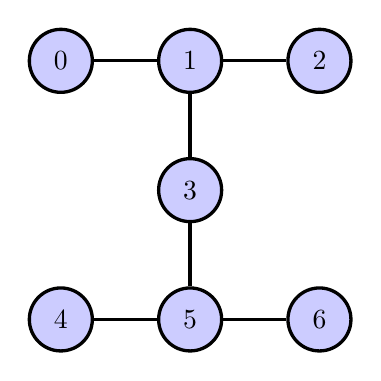
\begin{tikzpicture}
        \tikzset{
            node/.style={
                    very thick,
                    circle,
                    fill=blue!20,
                    draw,
                    minimum size=.8cm,
                }
        }
        \node[node] (0) {$0$};
        \node[node] (1) [right = .8cm of 0] {$1$};
        \node[node] (2) [right = .8cm of 1] {$2$};
        \node[node] (3) [below = .8cm of 1] {$3$};
        \node[node] (5) [below = .8cm of 3] {$5$};
        \node[node] (4) [left  = .8cm of 5] {$4$};
        \node[node] (6) [right = .8cm of 5] {$6$};

        \path[draw, very thick]
        (0) edge node {} (1)
        (1) edge node {} (2)
        (1) edge node {} (3)
        (3) edge node {} (5)
        (5) edge node {} (4)
        (5) edge node {} (6);
    \end{tikzpicture}
    \caption{IBMQ Jakarta Architecture}\label{fig:ibm-jakarta}
\end{figure}

We can now define the main problem of quantum circuit compilation: that of the qubit mapping problem.\footnote{This sometimes also goes by the name of the qubit routing problem, or qubit scheduling problem although sometimes these mean slightly different things.}
If we have both a quantum circuit $C\in G^*$, and a quantum computer with network topology $G$, can the computer perform our circuit?
In order to address this question we must first talk about universal gate sets.

\subsection{Universal Gate Sets}
In order to harness the full power of a quantum computer, we hope it to be able
\begin{definition}
    A gate set $G$ on $n$ qubits is called \emph{universal} if for all $U\in\U{2^n}$ there exists a circuit $C\in G^*$ such that $\mult(C) = U$.
\end{definition}

The question of which gate sets are universal for quantum computation is important both for our theoretical understanding of quantum computation, but also for building physical devices.
Examples that have been shown to be universal are
\begin{itemize}
    \item \CNOT{} plus $\U{2}$ as shown in~\cite{universal-cnot-u2}
    \item \CNOT{}, Hadamard, and the $\frac{\pi}{8}$-gate\footnote{The $\frac{\pi}{8}$-gate is also sometimes called $T$ and has matrix representation $\smqty[1 & 0 \\ 0 & \e^{\iu\pi/4}]$.} as shown in~\cite{universal-cnot-had-p8}
    \item \CCNOT{} (Toffoli), Hadamard, and the $\frac{\pi}{4}$-gate\footnote{The $\frac{\pi}{4}$-gate is also sometimes called $S$ and has matrix representation $\smqty[1 & 0 \\ 0 & \e^{\iu\pi/2}]$.} as shown in~\cite{universal-ccnot-had-p4}
    \item \CNOT{} plus any single qubit gate that does not preserve the computational basis and is not the Hadamard gate as shown in~\cite{universal-cnot-basis-change}
\end{itemize}

The authors in~\cite{universal-cnot-u2} also show

With these universal gate sets


% With these two definitions we can already formulate a very important question.
% Suppose we have a target unitary $U\in\U{2^n}$.
% Is there a circuit $C\in\free{G}$ such that $\dbrackets{C} = U$?
% hi
% If we'd like our circuit to implement a target unitary $U\in\U{2^n}$,
% In \cite{optimalSyn}
\cleardoublepage
% \ctparttext{Here we will cover the very basics of quantum computation.}
% \part{Quantum Computation}\label{pt:qomputation}
\ctparttext{You can put some informational part preamble text here.}
\part{Back End}\label{pt:qompilers}
%************************************************
\chapter{Quantum Hardware}\label{ch:hardware}
%************************************************

The goal of this chapter is twofold.
First we introduce the most common constraints seen in modern quantum hardware, as well as other common tools used to measure the effectiveness and efficacy of a given quantum computer.
Second we will introduce the mathematical formalism needed in order to formulate the problems related to quantum circuit compilation we will see in~\cref{ch:circuit-compilers}.

\section{Requirements}
As we saw in~\cref{sec:history} the first realization of a qubit happened in~\citeyear{firstqubit}.
A year later theoretical physicist David DiVincenzo published~\cite{divincenzo} where he outlined 5 requirements to make an effective quantum information processing device.
\begin{requirements}
    \item A scalable physical system with well characterized qubits.\label{req:scalable}
    \item The ability to initialize the state of the qubits to a simple fiducial state, such as $\ket{0}^{\otimes n}$.\label{req:initialize}
    \item Long, relevant decoherence times, much longer than the gate operation time.\label{req:Ttimes}
    \item A universal set of quantum gates.\label{req:universal}
    \item A qubit specific measurement capability.\label{req:measure}
\end{requirements}
While not an entirely revolutionary list at the time of writing,\todo{whose writing?} having concrete goals and checkpoints for the community to rally around/focus on meant maintainable, and trackable progress.
Again at the time of writing,~\cref{req:initialize,req:universal,req:measure} have mostly been taken care of and~\cref{req:Ttimes,req:scalable} are the areas we need the most improvement.

\section{Quantum Chips}

\begin{definition}
    A \emph{quantum chip's topology} is a graph $G = (V, E)$ with the vertices representing qubits, and edges representing connections between qubits where quantum gates of the correct arity can be applied.
\end{definition}

As an example take the the topology of IBM's \texttt{ibmq\_jakarta} shown in~\ref{fig:ibm-jakarta}~\cite{ibmq}.
``3'' being connected to ``1'' means that we can apply a 2-qubit unitary targeting both of those qubits, however the hardware does not support native 2-qubit gates between qubits ``2'' and ``6''.
\begin{figure}[ht]
    \centering
    \includestandalone[width=0.4\textwidth]{tikz/jakarta}
    \caption{IBMQ Jakarta Architecture}\label{fig:ibm-jakarta}
\end{figure}

We can now define the main problem of quantum circuit compilation: that of the qubit mapping problem.\footnote{This sometimes also goes by the name of the qubit routing problem, or qubit scheduling problem although sometimes these mean slightly different things.}
If we have both a quantum circuit $C\in G^*$, and a quantum computer with network topology $G$, can the computer perform our circuit?
In order to address this question we must first talk about universal gate sets.

% In \cite{optimalSyn}

\subsection{Hardware Specifications}

\subsubsection{Relaxation and Dephasing Times}\label{sec:Ttimes}

As qubits are two-state systems, they are often implemented experimentally using some physical system (\eg{} an atom) that has a ground state, and an excited state.
Excited states often have a tendency to ``decay'' into ground states, especially so when interacting with the environment.
Hence we define the \textbf{relaxation time}\footnote{This value also goes by the following names: coherence time, amplitude damping, longitudinal coherence time, spin lattice time, and spontaneous emission time.} $T_1$ as the lifetime for the state $\ket{1}$ decaying into $\ket{0}$.
This value can be experimentally found using the following methodology.
\begin{enumerate}
    \item Prepare the state $\ket{0}$
    \item Apply a Pauli $X$ gate to obtain $\ket{1}$
    \item Wait some time $t$ (during this time the qubit may decay into $\ket{0}$)
    \item Measure the qubit
\end{enumerate}
Each time we measure the qubit in the ground state we record the amount of time $t$ we waited.
This process is then modelled with an exponential decay of the form $\e^{-t/T_1}$.

The second important factor we need to understand is the \textbf{dephasing time}\footnote{Again, this value also goes by the following names: phase coherence time, phase damping, spin-spin relaxation time, transverse coherence time, and elastic scattering time.}
This time, instead of watching for the the bit flip from $\ket{1}$ to $\ket{0}$ we will watch for a phase flip from $\ket{+}$ to $\ket{-}$ via the following procedure.
\begin{enumerate}
    \item Prepare the state $\ket{0}$
    \item Apply a Hadamard $H$ gate to obtain $\ket{+}$
    \item Wait some time $t$ (during this time a phase might appear on either qubit)
    \item Apply another Hadamard $H$
    \item Measure the qubit
\end{enumerate}
Again, this experiment models an exponential decay with lifetime which we denote $T_2$.
This decoherence time is a measure of how quickly a superposition ($\ket{+}$) will decay into a classical mixture.
Since $T_1$ is a measure of how robust the qubit is against bit flips, and $T_2$ is a measure of how robust the qubit is against becoming probabilistic, these two quantities are very important track the progress of quantum computers.

\subsubsection{Gate Duration}

As qubits are finnicky beasts that don't want to retain their quantum-ness, how quickly we can perform gates is a very important measure and one tracked across many quantum computers.
This measure usually comes under the guise of \ac{CLOPS} first introduced in~\cite{clops}.

\subsubsection{Quantum Volume}

Now that we have seen how one might go about calibrating gates for a quantum computer, we must then ask: does individually calibrated gates imply a fully functional quantum computer?
Researchers have found that despite isolating qubits to the best of their ability, when sending instructions to a qubit (\eg{} a gate), nearby qubits can ``hear'' such a message and be affected by it~\cite{crosstalk,crosstalk2}.\todo{Are there other types of errors that make quantum volume worthwhile?}
With the introduction of errors that are not solely from a single qubit or gate, it makes sense to have a measure of how effective the quantum computer is as a whole.
\citeauthor{qvolume} introduce the notion of \textbf{quantum volume} designed to give a single number to measure the effectiveness of \ac{NISQ}-era quantum computers~\cite{qvolume}.
While understanding the full method to compute a quantum computer's quantum volume, the process consists of applying round of permutations $\pi$ of the qubits, followed by random elements of $\SU{4}$ as seen in~\cref{fig:qvolume}.

\begin{figure}[ht]
    \centering
    \begin{quantikz}
        & \gate[wires=4]{\pi}\gategroup[4,steps=2,style={dashed,rounded corners,fill=blue!20, inner xsep=2pt}, background]{Round 1} & \gate[wires=2]{\SU{4}} & \gate[wires=4]{\pi}\gategroup[4,steps=2,style={dashed,rounded corners,fill=blue!20, inner xsep=2pt}, background]{Round 2} & \gate[wires=2]{\SU{4}} & \ \ldots\ \qw & \gate[wires=4]{\pi}\gategroup[4,steps=2,style={dashed,rounded corners,fill=blue!20, inner xsep=2pt}, background]{Round $d$} & \gate[wires=2]{\SU{4}} & \qw \\
        &                     &                        &                     &                        & \ \ldots\ \qw &                     &                        & \qw \\
        &                     & \gate[wires=2]{\SU{4}} &                     & \gate[wires=2]{\SU{4}} & \ \ldots\ \qw &                     & \gate[wires=2]{\SU{4}} & \qw \\
        &                     &                        &                     &                        & \ \ldots\ \qw &                     &                        & \qw
    \end{quantikz}
    \caption{Quantum Volume Protocol}\label{fig:qvolume}
\end{figure}



\section{Errors}

Errors are ubiquitous in quantum computing and for the near future there is almost certainly no getting around them.
Not only are errors abundant, but they can vary across the chip, and they can very in type.
The first error that is often encountered is that of \textbf{gate errors}.
Some examples of gate errors might be
\begin{itemize}
    \item performing $R_X(\theta + \varepsilon)$ when you intended to do $R_X(\theta)$, or
    \item performing $H + \varepsilon X$ when you intended to apply $H$.
\end{itemize}
This first type of error is sometimes mitigated experimentally if $\varepsilon$ is either fixed, or coupled in some way to $\theta$.
However it may be the case that a more complex coupling is taking place dependent on the surrounding state of the qubit that the gate is acting on.
Since we represent a quantum chip as a graph, one way to quantify errors is to attach a number to each node and edge.
The node error rate represents the computers error rate on performing a single qubit unitary, and the edge represents the computers error rate for performing a 2-qubit unitary.

The next type of error that's important for circuit compilation is that of \textbf{\ac{SPAM}} errors. % TODO it's bolding the acro :(
Again each node on the computers chip can be assigned another number which denotes the computers error rate when performing a measurement.\todo{how to state prep. errors come into play?}

Finally we have cross-talk.\todo{can we even mitigate cross-talk with compilation?}

% ***********************************************
\chapter{Quantum Compilers}\label{ch:qcomps}
% ***********************************************

We can now return to the issue of compilers.
It should now be clear that the level of abstraction we work at when designing quantum algorithms is much higher than the capabilities of our current, and likely future hardware.
Hence quantum compilers are needed for two steps.
\begin{figure}[h]
    \centering
    \tikzset{
        frame/.style={
                draw,
                text width=6em,
                text centered,
                minimum height=4em,
                drop shadow,
                fill=orange!40,
                rounded corners,
            },
    }
    \begin{tikzpicture}[font=\sffamily, very thick, node distance=4cm]
        \node[align=center] (qa) {Quantum \\ Algorithm};
        % \node[frame, right of=qa] (compiler) {Compiler};
        \node[frame, right of=qa] (ir) {};%Intermediate \\ Representation};
        \node[align=center, above right=.5cm and 1cm of ir] (ha) {Hardware A};
        \node[align=center, below=.5cm of ha] (hb) {Hardware B};
        \node[align=center, below=.1cm of hb] (hdots) {\vdots};

        % \node[align=center, right of=compiler] (ml) {Hardware A};

        \draw[-stealth] (qa) -- (ir);
        \draw[-stealth] (ir) -- (ha);
        \draw[-stealth] (ir) -- (hb);
        % \draw[-stealth] (ir) -- (hdots);

        \node[very thick, draw=orange!20, fit=(ir), inner sep=3mm, label=above:{Quantum Compiler}, rounded corners](qcompiler) {};
    \end{tikzpicture}
    \caption{Action of Quantum Compiler}\label{fig:quantumcompiler}
\end{figure}

\dots Thus when compiling circuits, we need to minimize the number of \SWAP{} gates we must add since we saw in~\cref{eq:cnotswap} that each \SWAP{} takes 3 \CNOT{} gates.

\paragraph{Compiling the Toffoli Gate}
Since most hardware are not capable of 3-qubit operations we must decompose the Toffoli, or \CCNOT{} gate into something more manageable.
This is typically done using \CNOT{}'s, Hadamard's ($H$), and $\pi/8$ ($T$) gates~\cite{nielsenchuang}.
\begin{equation}
    \begin{quantikz}[column sep=.25cm]
        & \ctrl{1} & \midstick[3,brackets=none]{$=$} \qw & \qw      & \qw      & \qw              & \ctrl{2} & \qw      & \qw      & \qw              & \ctrl{2} & \qw      & \ctrl{1} & \gate{T}         & \ctrl{1} & \qw \\
        & \ctrl{1} & \qw                                 & \qw      & \ctrl{1} & \qw              & \qw      & \qw      & \ctrl{1} & \qw              & \qw      & \gate{T} & \targ{}  & \gate{T^\dagger} & \targ{}  & \qw \\
        & \targ{}  & \qw                                 & \gate{H} & \targ{}  & \gate{T^\dagger} & \targ{}  & \gate{T} & \targ{}  & \gate{T^\dagger} & \targ{}  & \gate{T} & \gate{H} & \qw              & \qw      & \qw
    \end{quantikz}
\end{equation}
This is an important decomposition as the \CCNOT{} gate appears in the modular exponentiation problem which is a core part of Shor's algorithm~\cite{shor-encryption}.
Hence if there are smaller decompositions than shown above that would be ideal as \emph{one} \CCNOT{} gate becomes 14!
\citeauthor{universal-cnot-u2} show a more compact decomposition of \CCNOT{} using only 3 \CNOT{} gates if the phase of one of the qubits is allowed to change~\cite{universal-cnot-u2}.
Let $G = R_Y(\frac{\pi}{4})$ in the following circuit. % following https://arxiv.org/pdf/quant-ph/9705009.pdf rather than original paper
\begin{equation}
    \begin{quantikz}%[column sep=.25cm]
        & \ctrl{1} & \midstick[3,brackets=none]{$\approx$} \qw & \qw                        & \qw      & \qw                        & \ctrl{2} & \qw                       & \qw      & \qw                       & \qw \\
        & \ctrl{1} & \qw                                       & \qw                        & \ctrl{1} & \qw                        & \qw      & \qw                       & \ctrl{1} & \qw                       & \qw \\
        & \targ{}  & \qw                                       & \gate{G^\dagger} & \targ{}  & \gate{G^\dagger} & \targ{}  & \gate{G} & \targ{}  & \gate{G} & \qw
    \end{quantikz}
\end{equation}
However the question ended in~\citeyear{toff3cnot} when it was shown that a true equality preserving decomposition of the \CCNOT{} gate requires a minimum of 6 \CNOT{} gates~\cite{toff3cnot}.\footnote{This result shows that a minimum of 6 \CNOT{} gates must be used, \textbf{if} they are being used. Other decompositions not using \CNOT{} gates might still be more compact.}

\section{Strong and Weak Compilation}


One of the benefits of the modular compiler structure seen in~\cref{fig:compends} is that once the optimizer is made, we can write a backend to go to real hardware, \textbf{and} write another backend to send the code to classical hardware.
This in effect provides an optimized quantum simulator.

\section{Compiling on a ring}

\section{Methods}

It's important to note there that quantum circuit compilers exist and in many of the references that follow the authors' proposed compilation methods are benchmarked against the most prevalent compiler Qiskit~\cite{qiskit}.

\paragraph{QAOA}
Compilers have also been built to attack specific problems such as the \ac{QAOA}~\cite{qaoa} where particular gates can be swapped horizontally in circuit diagrams due to their commutative nature.
Focusing in this particular problem, the authors in~\cite{qaoa-compiler} have been able to reduce the gate count by 23\% and circuit depth by 53\% on average.
In the future we might hope to build these problem specific compilers into a more general purpose one that can diagnose and understand when to use problem specific compilers on demand.

\paragraph{VQE}
Another hybrid quantum-classical algorithm that has seem much attention is that of the \ac{VQE}~\cite{vqe,vqe2}.
This algorithm is used in quantum chemistry to calculate the ground state of a molecular Hamiltonian using a parametrized quantum circuit as a cost function, and the classical compute nodes as an optimizer.
\Eg{} let $\boldsymbol{\theta} \in \R^n$ be a vector of numbers that our circuit $U$ depends on, \ie{} $U: \R^n \to \U{2^m}$ for some number of qubits $m$.
\begin{figure}[ht] % TODO label positioning fucked
    \centering
    \includestandalone[width=0.8\textwidth]{tikz/vqe}
    \caption{\acs{VQE} Schematic}\label{fig:vqe}
\end{figure}
A compiler specific to this problem has been created, and generalized to further quantum-classical algorithms in~\cite{vqe-compiler} and the authors have leveraged much of the existing infrastructure brought forth by the LLVM project discussed in~\cref{sec:llvm}.
This allows the classical optimizations to be handled by the robust LLVM system, while using new circuit compilation techniques on the variational circuit.


\section{Quantum Stack}

% ******************************************************
% Back matter
% ******************************************************
\appendix
%\renewcommand{\thechapter}{\alph{chapter}}
\cleardoublepage
\part{Appendix}
% ***********************************************
% Appendix
% ***********************************************

\chapter{Appendix Test}

\section{Appendix Section Test}

% ******************************************************
% Other Stuff in the Back
% ******************************************************
\cleardoublepage\include{aux/bibliography}
\cleardoublepage%*******************************************************
% Declaration
%*******************************************************
\pdfbookmark[0]{Declaration}{declaration}
\chapter*{Declaration}
\thispagestyle{empty}
This thesis consists of material all of which I authored.

I understand that my thesis may be made electronically available to the public.
\bigskip

\noindent\textit{\myLocation, \myTime}

\smallskip

\begin{flushright}
    \begin{tabular}{m{5cm}}
        \\ \hline
        \centering\myName \\
    \end{tabular}
\end{flushright}

\cleardoublepage\pagestyle{empty}

\hfill

\vfill

\pdfbookmark[0]{Colophon}{colophon}
\section*{Colophon}
This document was typeset using the typographical look-and-feel \texttt{classicthesis} developed by Andr\'e Miede and Ivo Pletikosić.
The style was inspired by Robert Bringhurst's seminal book on typography ``\emph{The Elements of Typographic Style}'' and is available at:
\begin{center}
    \url{https://bitbucket.org/amiede/classicthesis/}
\end{center}

Hermann Zapf's \emph{Palatino} and \emph{Euler} type faces are used and the ``typewriter'' text is typeset in \emph{Bera Mono}.



\end{document}
